{% -*- mode: LaTeX; TeX-PDF-mode: t; TeX-master: "manual"; -*-
}

\begin{example}
\label{sec:eiol:examples:1}
%
The following is an example of
\xmlstructref{eiout}{printonconsolecommand} using different
\xmlstructref{eiout}{content} environments with different formats:

\medskip
\begin{lstlisting}
<printonconsole consoleid="1" consoletitle="Welcome">
  <content format="text">
    Hello World
  </content>
  <content format="html">
    <span style="color: red;">Hello</span> World
  </content>
  <content format="svg">
    <svg height="100" width="100">
      <circle cx="50" cy="50" r="40" fill="red" />
    </svg> 
  </content>
</printonconsole>
\end{lstlisting}

\medskip
\noindent
Its execution in the web-client generates the output depicted in
Figure~\ref{fig:examples:1}.

\begin{figure}[h]
\hrule\smallskip
\begin{center}
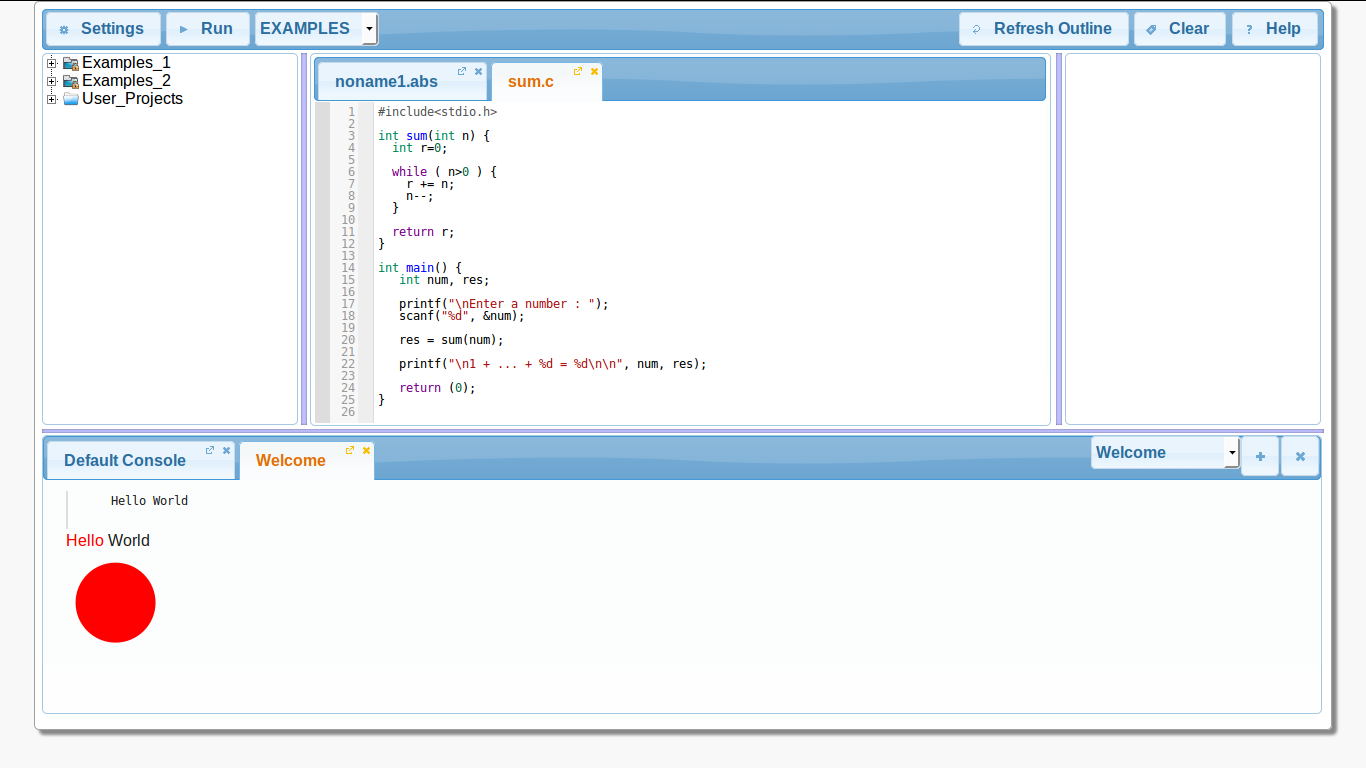
\includegraphics[width=1\textwidth]{fig/example1.png}
\end{center}
\caption{Output of Example~\ref{sec:eiol:examples:1}}
\label{fig:examples:1}
\hrule
\end{figure}
\end{example}

\begin{example}
\label{sec:eiol:examples:2}
%
The following is an example of
\xmlstructref{eiout}{oncodelineclickaction} which executes two
\xmlstructref{eiout}{highlightlinescommand}, each with different
\xmlstructattr{outclass}:

\medskip
\begin{lstlisting}
<eiactions>
 <oncodelineclick>
  <lines> <line from="3" /> </lines>
  <eicommands>
   <highlightlines outclass="info">
    <lines> <line from="2" to="4" /> </lines>
   </highlightlines>
   <highlightlines outclass="warning">
    <lines> <line from="6" fromch="4" toch="8" /> </lines>
   </highlightlines>
  </eicommands>
 </oncodelineclick>
</eiactions>
\end{lstlisting}

\medskip
\noindent
Its execution in the web-client generates the output depicted in
Figure~\ref{fig:examples:2}. Note that a click on the arrow (in the
left-side gutter) executes the commands and another click undo their
corresponding effect.


\begin{figure}[h]
\hrule\smallskip
\begin{center}
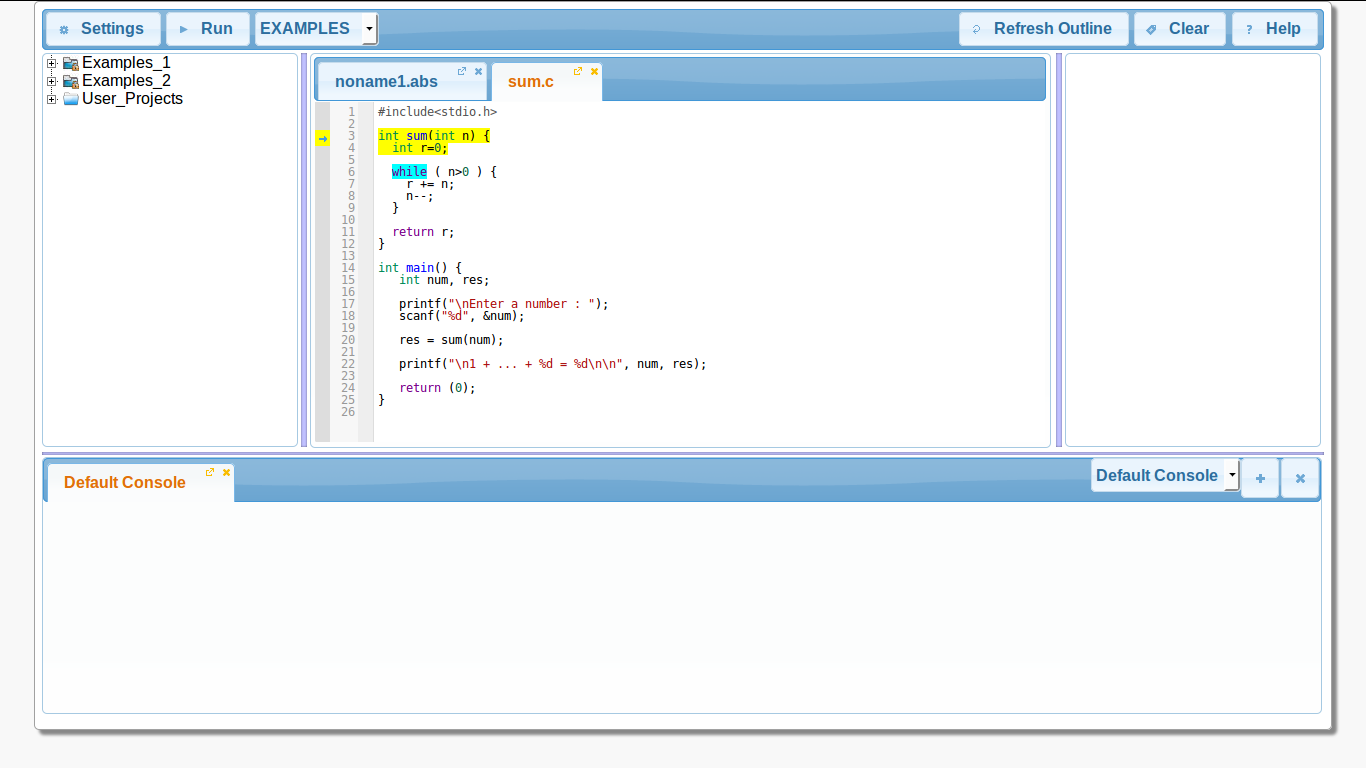
\includegraphics[width=1\textwidth]{fig/example2.png}
\end{center}
\caption{Output of Example~\ref{sec:eiol:examples:2}}
\label{fig:examples:2}
\hrule
\end{figure}
\end{example}


\begin{example}
\label{sec:eiol:examples:3}

The following is an example of \xmlstructref{eiout}{dialogboxcommand},
using a \xmlstructref{eiout}{content} environment with \lst{graph}
format.

\medskip
\begin{lstlisting}
<dialogbox boxtitle="CPU use" boxwidth="800" boxheight="500">
  <content format="graph">
    { "title":"BFS - Acer G5453",
      "f-titles":["Time","% CPU","% Mem"],
      "y-title":"%",
      "x-title":"Time",
      "groups":["BFS"],
      "labels":["Acer","G5453"],
      "values":[[1,22,43],[2,40,47],[3,82,88],[4,40,75]]
    }
    { "title":"BFS - Acer B12",
      "f-titles":["Timee","% CPU","% Mem"],
      "y-title":"%",
      "x-title":"Time",
      "groups":["BFS"],
      "labels":["Acer","B12"],
      "values":[[1,42,66],[2,65,47],[3,99,91],[4,68,92]]
    }
  </content>
</dialogbox>
\end{lstlisting}

\medskip
\noindent
Its execution in the web-client generates the output depicted in
Figure~\ref{fig:examples:3}.

\begin{figure}[h]
\hrule\smallskip
\begin{center}
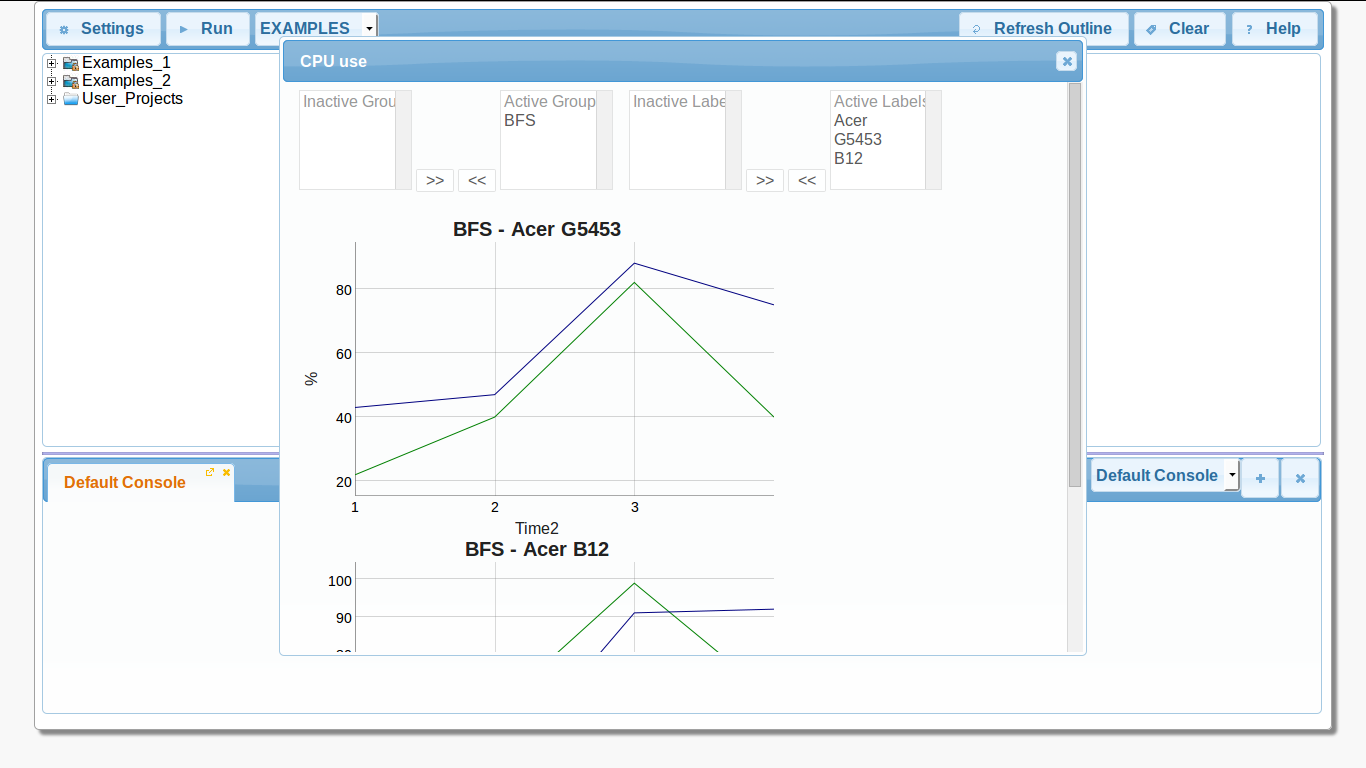
\includegraphics[width=1\textwidth]{fig/example3.png}
\end{center}
\caption{Output of Example~\ref{sec:eiol:examples:3}}
\label{fig:examples:3}
\hrule
\end{figure}

\begin{example}
\label{sec:eiol:examples:4}
%
The following is an example of \xmlstructref{eiout}{writefilecommand},
which adds a new file to the file-manager:

\medskip
\begin{lstlisting}
<writefile filename="dir1/newfile.cpp" overwrite="false">
<![CDATA[
#include <iostream>
using namespace std;
int main(){
  cout << "Hello World!" << endl;
  return 0;
}
]]>
</writefile>
\end{lstlisting}

\medskip
\noindent
Note the of \lst{<![CDATA[ ... ]]>}, this is necessary due to the use
of plain-text with special characters. Its execution in the web-client
generates the output depicted in Figure~\ref{fig:examples:4}.

\begin{figure}[h]
\hrule\smallskip
\begin{center}
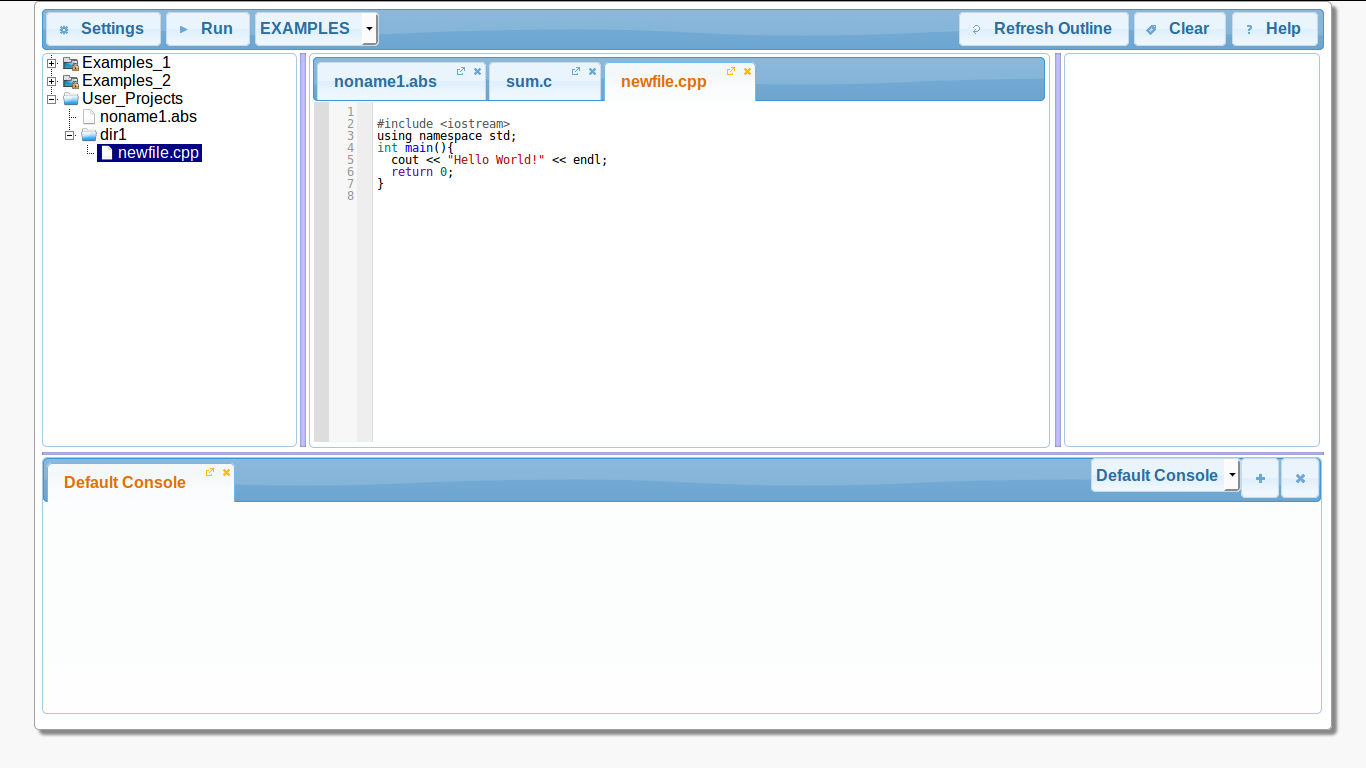
\includegraphics[width=1\textwidth]{fig/example4.png}
\end{center}
\caption{Output of Example~\ref{sec:eiol:examples:4}}
\label{fig:examples:4}
\hrule
\end{figure}
\end{example}

\end{example}

\begin{example}
\label{sec:eiol:examples:5}
%
The following is an example of \xmlstructref{eiout}{setcsscommand},
together with an action \xmlstructref{eiout}{onclickaction} which
changes the size of some text when it is clicked:

\medskip
\begin{lstlisting}
<eicommands>
 <printonconsole>
  <content format="html">
   <div id="wrap">
    <span>(*Some text*)</span><br/>
    <span id="text">Click me!</span><br/>
   </div> 
  </content>
 </printonconsole>
</eicommands>
<eiactions>
 <onclick>
  <elements>
   <selector value="#text" />
  </elements>
  <eicommands>
   <setcss>
    <elements>
     <selector value="#text" />
    </elements>
    <cssproperties>
     <cssproperty name="font-size" value="30px" />
    </cssproperties>
   </setcss>
  </eicommands>
 </onclick>
</eiactions>
\end{lstlisting}

\medskip
\noindent
Its execution in the web-client generates the output depicted in
Figure~\ref{fig:examples:5} -- it includes the result after clicking
on the text ``\lst{Click me!}''.

\begin{figure}[h]
\hrule\smallskip
\begin{center}
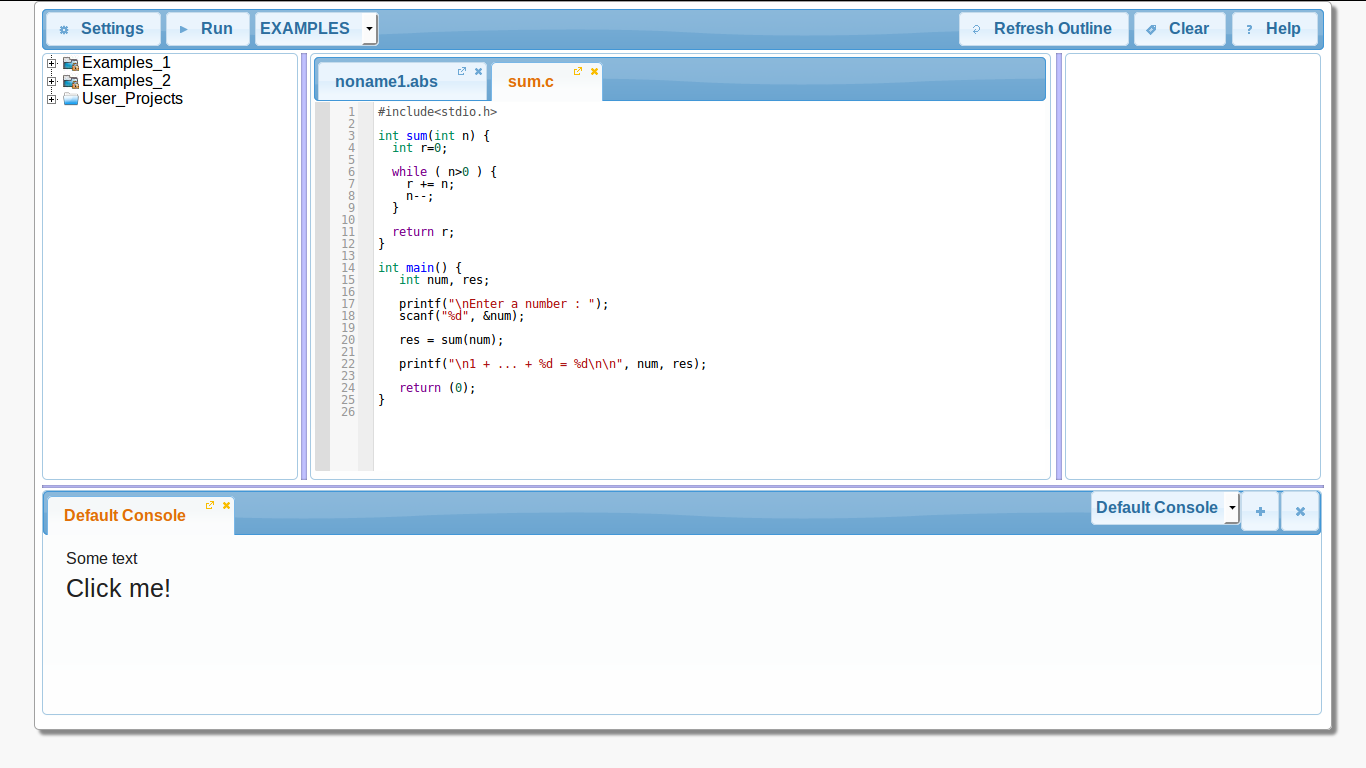
\includegraphics[width=1\textwidth]{fig/example5.png}
\end{center}
\caption{Output of Example~\ref{sec:eiol:examples:5}}
\label{fig:examples:5}
\hrule
\end{figure}
\end{example}

\begin{example}
\label{sec:eiol:examples:6}
%
The following is an example of
\xmlstructref{eiout}{changecontentcommand}. Assuming that we add the
following command to the list of commands of the
\xmlstructref{eiout}{onclickaction} in
Example~\ref{sec:eiol:examples:5}, it will add some text to the HTML
tag with identifier \lst{wrap} when ``\lst{Click me!}'' is clicked:

\medskip
\begin{lstlisting}
<changecontent action="append">
 <elements>
  <selector value="#wrap"/>
 </elements>
 <content format="html">
  <span style="color:red;">New Text added </span><br/>
 </content>
</changecontent> 
\end{lstlisting}

\medskip
\noindent
Its execution in the web-client generates the output depicted in
Figure~\ref{fig:examples:6} (after clicking on ``\lst{Click me!}'').

\begin{figure}[h]
\hrule\smallskip
\begin{center}
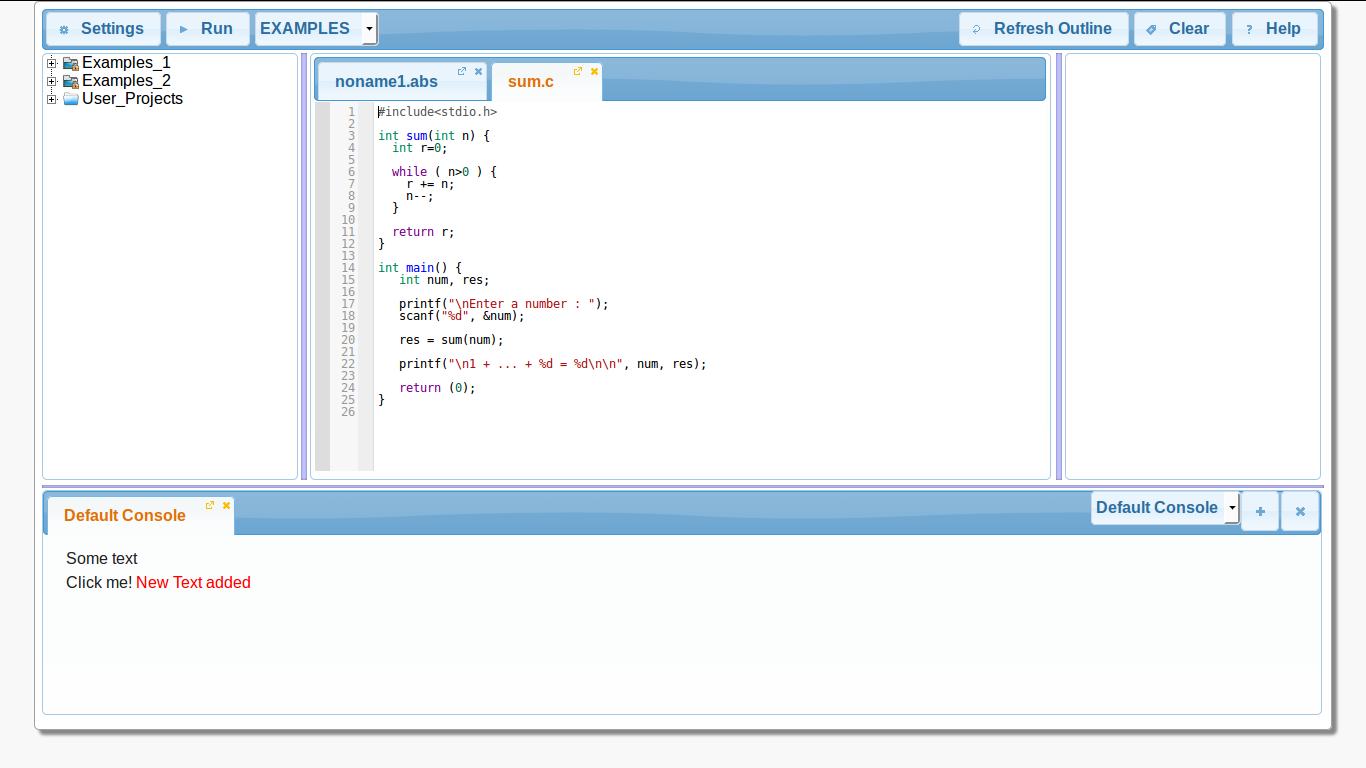
\includegraphics[width=1\textwidth]{fig/example6.png}
\end{center}
\caption{Output of Example~\ref{sec:eiol:examples:6}}
\label{fig:examples:6}
\hrule
\end{figure}
\end{example}

\begin{example}
\label{sec:eiol:examples:7}
%
The following is an example of \xmlstructref{eiout}{addmarkercommand},
using different \xmlstructattr{outclass} values:

\medskip
\begin{lstlisting}
<addmarker outclass="info">
 <lines>
  <line from="2" />
 </lines>
 <content format="text">
  Information
 </content>
</addmarker>
<addmarker outclass="warning">
 <lines>
  <line from="4" />
 </lines>
 <content format="text">
  Warning
 </content>
</addmarker>
<addmarker outclass="error">
 <lines>
  <line from="6" />
 </lines>
 <content format="text">
  Error
 </content>
</addmarker>
\end{lstlisting}

\medskip
\noindent
Its execution in the web-client generates the output depicted in
Figure~\ref{fig:examples:7}.

\begin{figure}[h]
\hrule\smallskip
\begin{center}
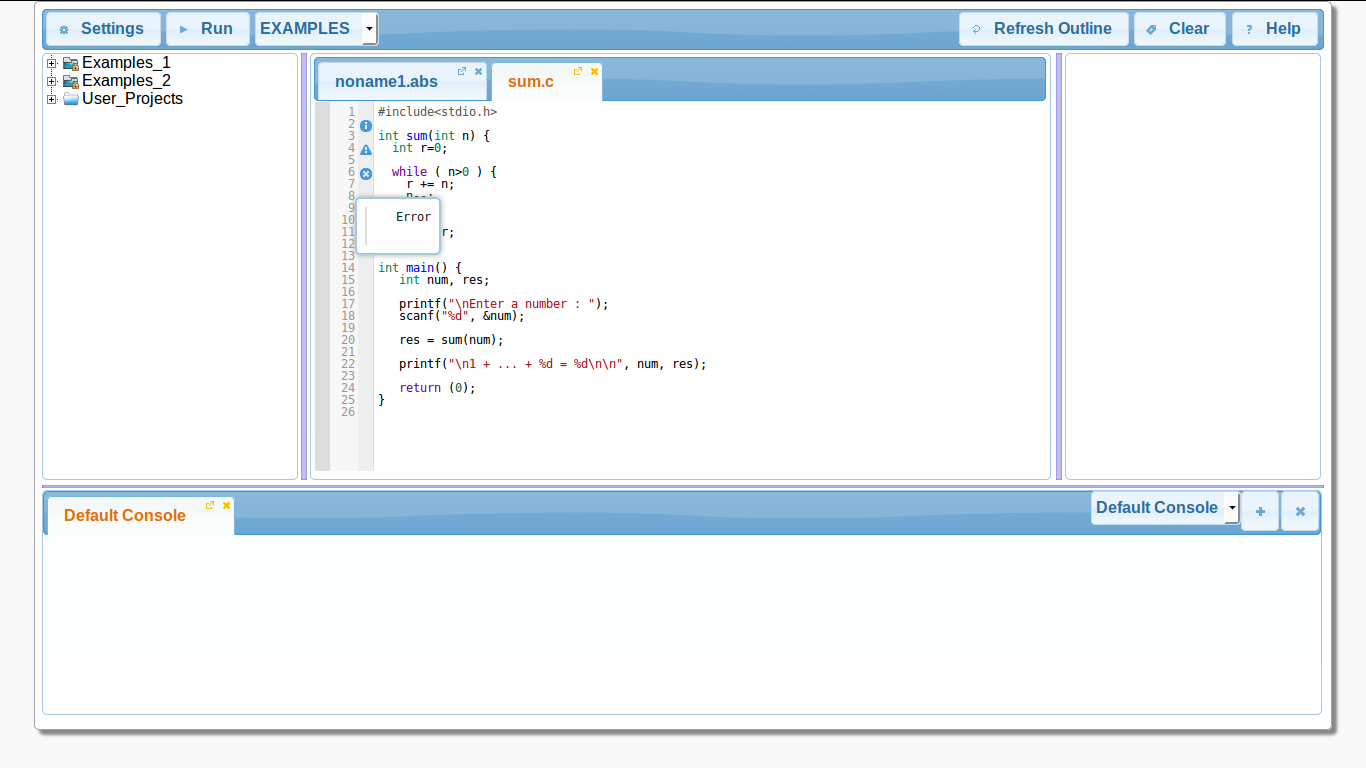
\includegraphics[width=1\textwidth]{fig/example7.png}
\end{center}
\caption{Output of Example~\ref{sec:eiol:examples:7}}
\label{fig:examples:7}
\hrule
\end{figure}
\end{example}

\begin{example}
\label{sec:eiol:examples:8}
%
The following is an example of 
\xmlstructref{eiout}{addinlinemarkercommand} using different
\xmlstructattr{outclass} values:

\medskip
\begin{lstlisting}
<addinlinemarker outclass="info">
 <lines>
  <line from="2" />
 </lines>
 <content format="text">
  Information
 </content>
</addinlinemarker>
<addinlinemarker outclass="warning">
 <lines>
  <line from="4" />
 </lines>
 <content format="text">
  Warning
 </content>
</addinlinemarker>
<addinlinemarker outclass="error">
 <lines>
  <line from="6" />
 </lines>
 <content format="text">
  Error
 </content>
</addinlinemarker>
\end{lstlisting}

\medskip
\noindent
Its execution in the web-client generates the output depicted in
Figure~\ref{fig:examples:8}.

\begin{figure}[h]
\hrule\smallskip
\begin{center}
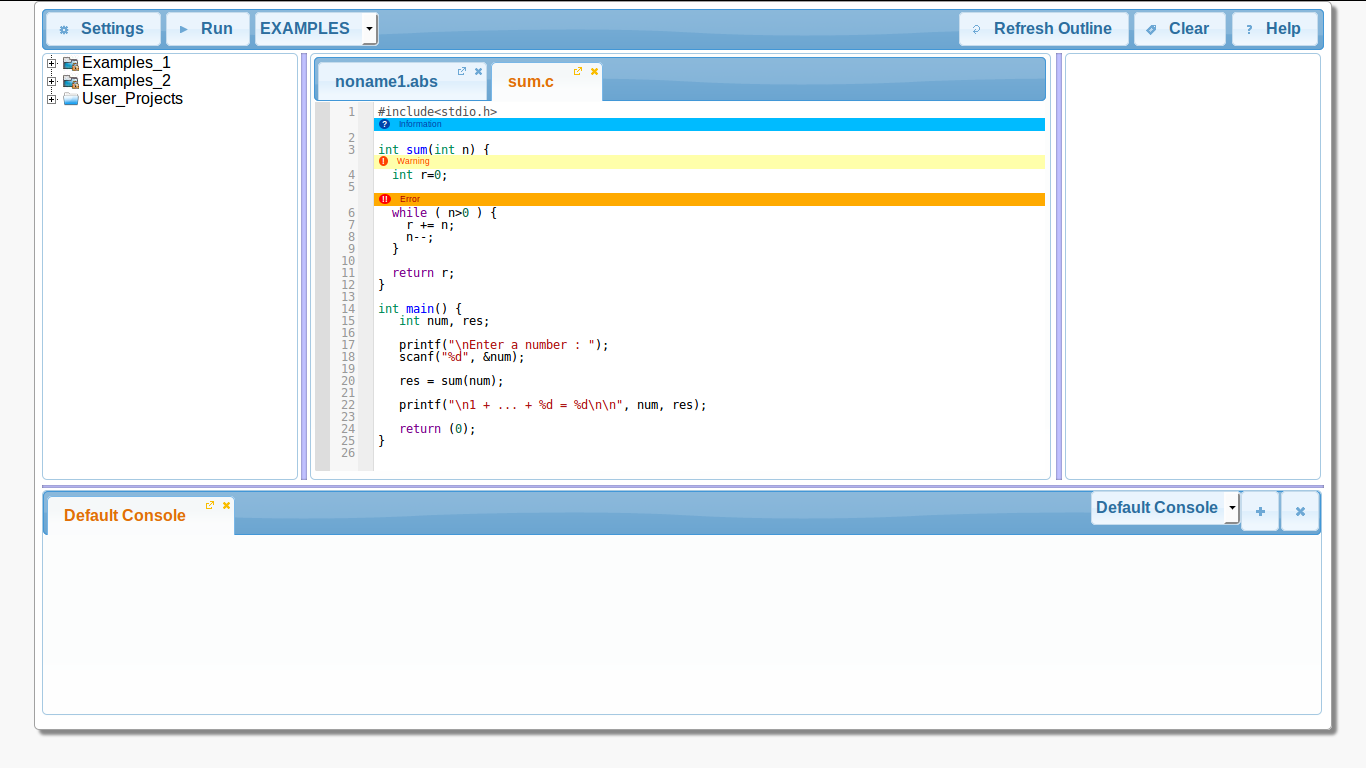
\includegraphics[width=1\textwidth]{fig/example8.png}
\end{center}
\caption{Output of Example~\ref{sec:eiol:examples:8}}
\label{fig:examples:8}
\hrule
\end{figure}
\end{example}

\begin{example}
\label{sec:eiol:examples:9}
%
The following is an example of \xmlstructref{eiout}{downloadcommand},
to download a file called \lst{$\mbox{download.test}$} generated by a
tool execution with \emph{execution identifier} \lst{xV54fga}:

\medskip
\begin{lstlisting}[mathescape=false]
<download execid="xV54fga" filename="download.test" />
\end{lstlisting}
%$
\medskip
\noindent
Its execution in the web-client generates the output as in
Figure~\ref{fig:examples:9}.

\begin{figure}[h]
\hrule\smallskip
\begin{center}
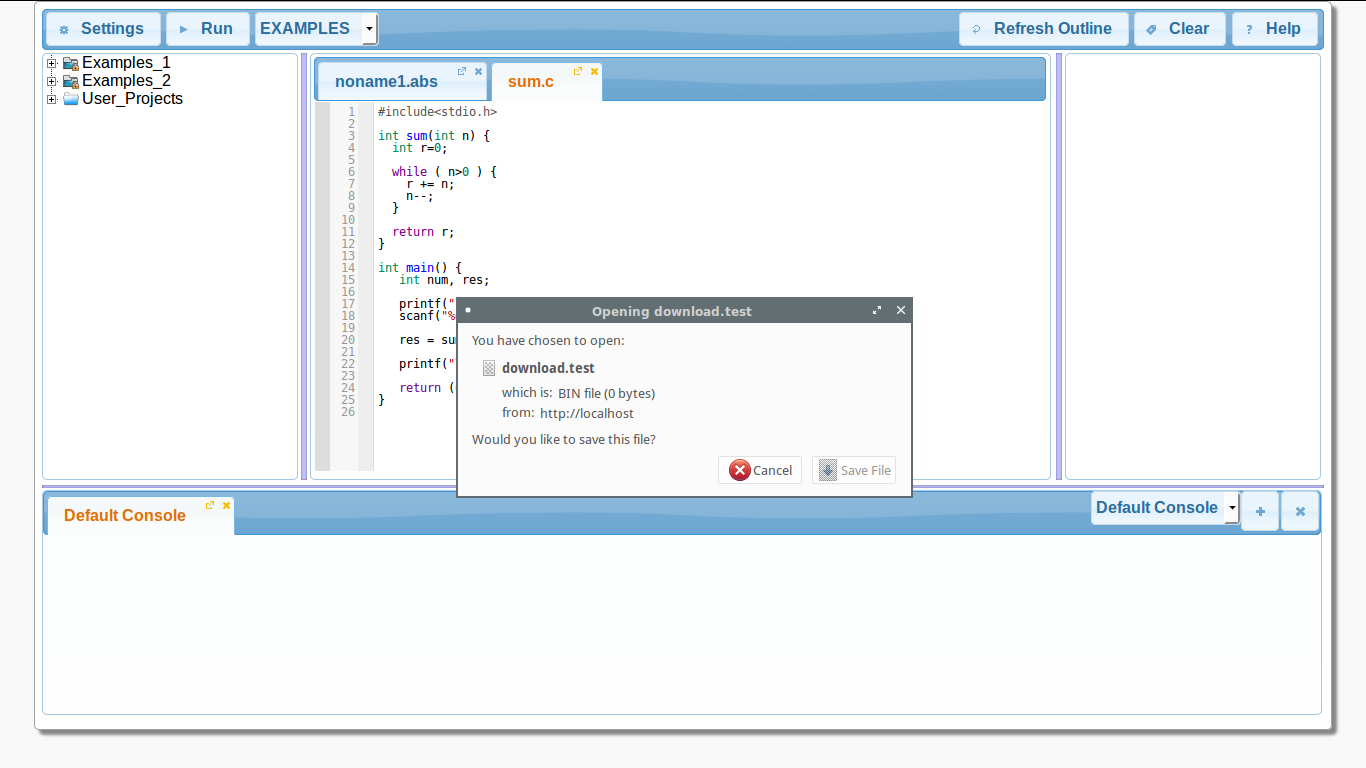
\includegraphics[width=1\textwidth]{fig/example9.png}
\end{center}
\caption{Output of Example~\ref{sec:eiol:examples:9}}
\label{fig:examples:9}
\hrule
\end{figure}
\end{example}

